\section{Methods}

\subsection{Phosphene Simulation Framework}
To assess SCAPE under conditions that approximate clinical prosthetic vision we employ the simulator of van der Grinten et al.\ \cite{vanderGrinten2024}. This pipeline models key aspects of cortical stimulation, including the retinotopic projection of electrodes into visual-field coordinates and the rendering of each electrode’s percept as a Gaussian phosphene. The resulting phosphene image captures the spatial layout of perceptual activations and serves as the input for SCAPE’s adaptive encoding stages.


\subsubsection{Electrode Placement}
We begin with \(E\) electrodes implanted in cortical tissue, each with a two-dimensional coordinate on the cortical surface:
\[
\{(x_i,y_i)\}_{i=1}^E.
\]
These positions are obtained from clinical implant schematics or patient-specific models.


\subsubsection{Retinotopic Projection and Phosphene Centers}
Each cortical electrode \((x_i,y_i)\) is mapped into visual-field coordinates \((\mu_{x,i},\mu_{y,i})\) using the inverse of the Wedge–Dipole transform introduced by Polimeni \emph{et al.}\ \cite{Polimeni2006}. This model captures cortical magnification, in which the foveal region is allocated a larger cortical representation than the periphery. In complex notation the forward mapping from visual-field polar coordinates \((r,\theta)\) to cortical coordinate \(w\) is
\[
w = k\bigl[\ln\bigl(r\,e^{i\alpha\theta} + a\bigr) 
       - \ln\bigl(r\,e^{i\alpha\theta} + b\bigr)\bigr],
\]
where \(r\) is eccentricity in degrees, \(\theta\) is polar angle, \(k\) scales degrees to cortical millimeters, and \(a,b,\alpha\) are fitted parameters. Analytically inverting this relation yields
\[
r\,e^{i\alpha\theta}
  = \frac{b\,e^{\phi} - a}{1 - e^{\phi}},
\quad
\phi = \frac{w}{k},
\]
from which
\[
r = \bigl|\tfrac{b\,e^{\phi} - a}{1 - e^{\phi}}\bigr|,
\quad
\theta = \frac{1}{\alpha}\arg\!\bigl(\tfrac{b\,e^{\phi} - a}{1 - e^{\phi}}\bigr).
\]
Applying this inverse transform to each \((x_i,y_i)\) and adding optional Gaussian angular noise and dropout produces \(N\le E\) phosphene centers
\[
\{(\mu_{x,i},\mu_{y,i})\}_{i=1}^N,
\]
expressed in degrees of visual angle. These centers form the basis for SCAPE’s density estimation and adaptive filtering \cite{vanderGrinten2024}.



\subsubsection{Gaussian Blob Rendering}
Empirical reports indicate that electrically evoked phosphenes are most often perceived as localized flashes of light with an approximately circular appearance \cite{vanderGrinten2024}. Although some studies describe elongated or irregular forms, for simplicity we model each phosphene as an isotropic Gaussian. Note that SCAPE’s core computations (density estimation and adaptive filtering) rely only on phosphene centers; the Gaussian shape is used downstream for visualization, evaluation, and amplitude normalization.

Formally, each phosphene center \((\mu_{x,i},\mu_{y,i})\) in visual‐field coordinates generates a two‐dimensional Gaussian blob
\[
G_i(x,y)
=
\exp\!\Bigl(-\frac{(x-\mu_{x,i})^2 + (y-\mu_{y,i})^2}{2\,\sigma^2}\Bigr),
\]
where \((x,y)\) are degrees of visual angle and \(\sigma\) is the nominal phosphene radius. The simulator rasterizes these Gaussians onto a regular image grid by converting \((\mu_{x,i},\mu_{y,i})\) into pixel positions according to the chosen field‐of‐view and resolution, evaluating \(G_i\) at every grid point, and summing across all \(N\) phosphenes:
\[
I_{\mathrm{raw}}(x,y)
=
\sum_{i=1}^{N} G_i(x,y).
\]
This raw phosphene map is then used for visualization, metric evaluation, and amplitude equalization but does not influence SCAPE’s density or filter‐scale computations.


\subsubsection{Amplitude Equalization}
Phosphene brightness varies with local electrode density and current spread, causing some regions to appear disproportionately bright or dim. To counteract this and present a uniform perceptual dynamic range, we apply a simple gain‐learning step after simulation.

Each phosphene \(i\) has an initial amplitude \(A_i=1\). We render the raw phosphene map \(I_{\mathrm{raw}}(x,y)\) and measure the peak intensity of each blob,
\[
m_i = \max_{x,y}\;G_i(x,y).
\]
We then adjust amplitudes by minimizing the squared error to a target intensity \(m^*\):
\[
\mathcal{L}(A) = \frac{1}{N}\sum_{i=1}^N \bigl(A_i\,m_i - m^*\bigr)^2.
\]
Starting from \(A_i=1\), we update each gain by gradient descent with learning rate \(\eta\) and clamp \(A_i\) to the interval \([A_{\min},A_{\max}]\). After a fixed number of iterations, the normalized map
\[
I_{\mathrm{norm}}(x,y)
=
\sum_{i=1}^N A_i\,G_i(x,y)
\]
has phosphenes with comparable peak brightness, improving visual consistency for evaluation and downstream decoding.  



\subsection{SCAPE Adaptive Encoding}

The fundamental challenge in cortical prosthetic vision is that electrode arrays sample the visual field nonuniformly. Regions with dense electrode coverage can resolve fine detail while sparse regions cannot. SCAPE addresses this by adapting image filtering to the local sampling density. First, we estimate a continuous density map from the simulator-derived phosphene centers. Next, we convert density into a spatial scale map via sampling-theorem principles. Finally, we apply a shift-variant filter whose parameters vary continuously across the image. This adaptive encoding preserves maximal detail where it is supported and reduces visual clutter where it is not.

\begin{figure}[ht]
  \centering
  % scale to 0.55 of the line width
  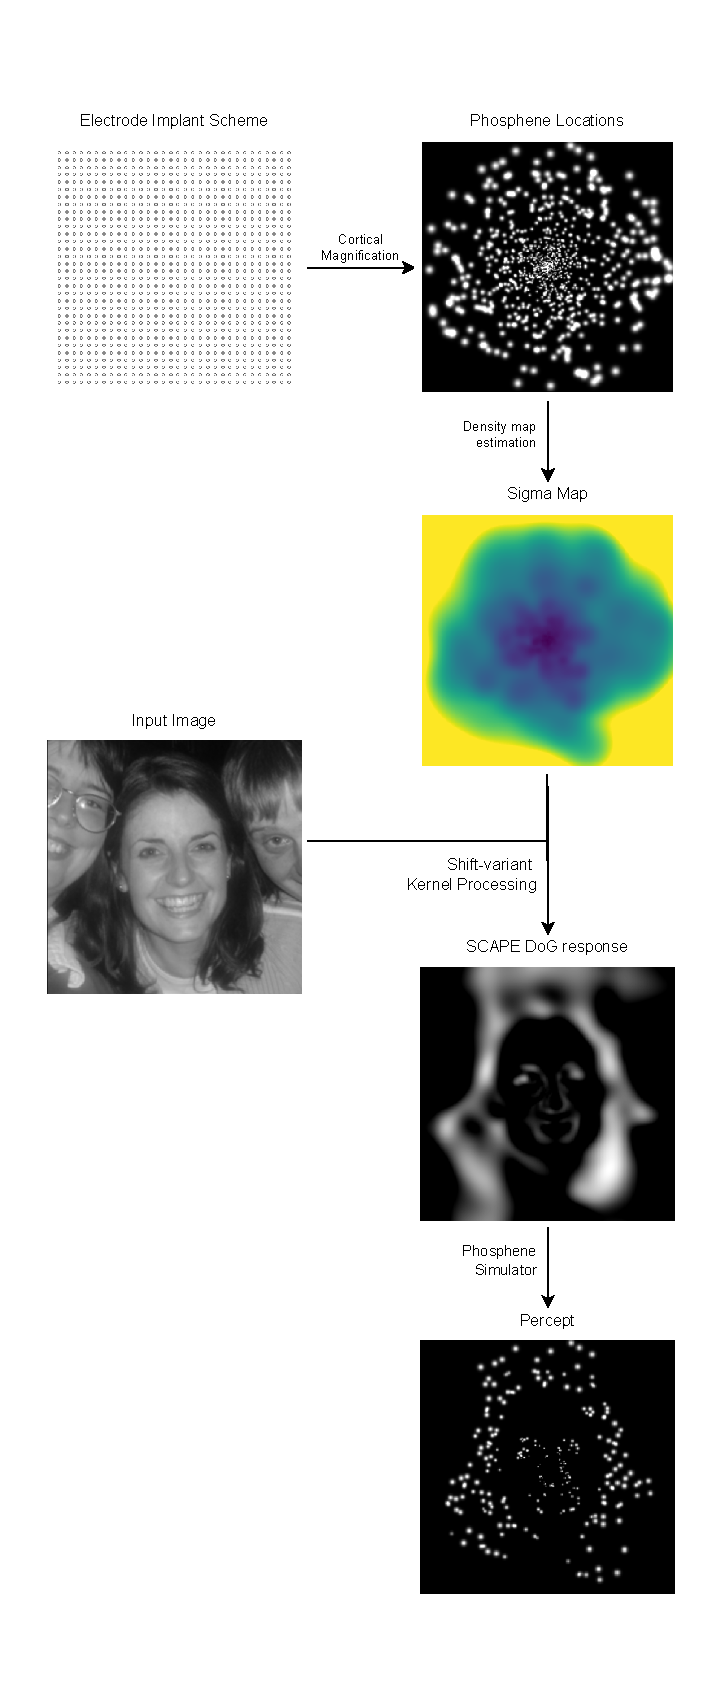
\includegraphics[width=0.9\linewidth]{figures/SCAPE.drawio.pdf}
  \caption{Overview of the SCAPE pipeline. Starting from a cortical implant layout (top left) we obtain phosphene centers via the simulator, estimate a local density map, convert it into a spatial scale ($\sigma$) map, and then apply shift-variant filtering to produce an activation map for phosphene rendering.}
  \label{fig:scape_pipeline}
\end{figure}

Figure~\ref{fig:scape_pipeline} illustrates the full SCAPE pipeline at a glance: from electrode layout to phosphene centers (Panel 1), to density and $\sigma$‐mapping (Panels 2–3), to the final shift‐variant filter output (Panel 4).  



\subsubsection{Density Estimation}
To guide adaptive filtering, SCAPE first computes a smooth sampling density \(d(x,y)\) over the visual field. This density reflects how densely the implant probes each region and sets the local spatial resolution limit. Two practical estimators are used.

\paragraph{Analytic Cortical Magnification}  
In an idealized implant that uniformly samples cortex around the fovea, one can predict density purely from known retinotopy. Writing eccentricity \(r=\sqrt{x^2+y^2}\) in degrees, the dipole‐model magnification  
\[
M(r)=\frac{k}{2\pi}\Bigl(\frac{1}{r+a}-\frac{1}{r+b}\Bigr)
\]
(with parameters \(k,a,b\) fit to human data \cite{vanderGrinten2024}) gives a nominal density  
\[
d_{\mathrm{analytic}}(x,y)=\frac{M(r)}{r}.
\]
We then scale \(d_{\mathrm{analytic}}\) so that its integral equals the total number of phosphenes \(N\):
\[
\iint d_{\mathrm{analytic}}(x,y)\,\mathrm{d}x\,\mathrm{d}y = N.
\]

\paragraph{Adaptive Kernel Density Estimation}  
For real implants with nonuniform phosphene layouts, we derive density directly from the simulator‐produced phosphene centers \(\{(\mu_{x,i},\mu_{y,i})\}\). We place a two‐dimensional Gaussian kernel at each center, choosing its bandwidth \(h_i\) based on local spacing. Specifically, let \(d_{(i,k)}\) be the distance from point \(i\) to its \(k\)th nearest neighbor; then
\[
h_i = \alpha\,d_{(i,k)},
\]
where \(\alpha\) (typically 1.0) controls smoothing. The density is
\[
d_{\mathrm{KDE}}(x,y)
= \sum_{i=1}^N \frac{1}{2\pi\,h_i^2}
\exp\!\Bigl(-\frac{(x-\mu_{x,i})^2 + (y-\mu_{y,i})^2}{2\,h_i^2}\Bigr).
\]
Finally we normalize so that
\[
\iint d_{\mathrm{KDE}}(x,y)\,\mathrm{d}x\,\mathrm{d}y = N.
\]
This adaptive KDE provides a flexible density estimate that captures local variations in electrode coverage.


\subsubsection{\(\sigma\)-Mapping via Nyquist Principles}
Once a smooth density map \(d(x,y)\) is available, SCAPE computes a corresponding spatial scale map \(\sigma(x,y)\) that specifies the width of the local filter. By the Nyquist sampling theorem \cite{Nyquist1928}, the highest spatial frequency resolvable at \((x,y)\) is
\[
f_{\mathrm{Nyq}}(x,y)
=\tfrac{1}{2}\sqrt{\frac{d(x,y)}{\pi}},
\]
since a local density of \(d\) phosphenes per unit area implies an average spacing of \(\sqrt{1/d}\). To suppress frequencies above \(f_{\mathrm{Nyq}}\), we choose a Gaussian filter whose standard deviation satisfies
\[
\sigma(x,y)
= \frac{\kappa}{f_{\mathrm{Nyq}}(x,y)}
= 2\,\kappa\sqrt{\frac{\pi}{d(x,y)}},
\]
where \(\kappa\) is a tuning constant (typically \(\kappa=1\)) that controls the cutoff sharpness. This mapping ensures that filter width increases in regions of low density, reducing visual clutter where detail cannot be resolved, and decreases in regions of high density, preserving fine structure.


\subsubsection{Shift-variant Filtering}
Having obtained a continuous filter‐scale map \(\sigma(x,y)\), SCAPE applies spatially adaptive filtering to the input image. At each location \((x,y)\), a local kernel \(K(\cdot;\sigma(x,y))\) is convolved with the image, yielding an output
\[
I_{\mathrm{filt}}(x,y)
=\iint K\bigl(u,v;\sigma(x,y)\bigr)\,
I_{\mathrm{in}}(x-u,y-v)\,\mathrm{d}u\,\mathrm{d}v.
\]
By tying the kernel’s parameters to the local sampling density, shift‐variant filtering preserves fine detail where electrodes are dense and reduces clutter where they are sparse. In the following sections we describe a concrete implementation using a difference of Gaussians and discuss how other kernel families can be incorporated within the same framework.


\paragraph{Difference-of-Gaussians Example}
As a concrete illustration of SCAPE’s adaptive filtering, we approximate the Laplacian-of-Gaussian (LoG) operator, widely used to model center–surround receptive fields in early vision \cite{Young1987}, with a pair of Gaussian kernels.  At each location \((x,y)\), the LoG of the input image \(I\) would be
\[
\mathrm{LoG}_{\sigma}(x,y)
=\nabla^2\bigl[G_{\sigma} * I\bigr](x,y),
\]
where \(G_{\sigma}\) is a Gaussian of standard deviation \(\sigma(x,y)\) and \(*\) denotes convolution.  Computing a full LoG at every pixel with its own \(\sigma\) has complexity \(\mathcal{O}(n^2)\) per pixel, where \(n\) is the kernel size, making it impractical for real-time use.  Instead, we approximate it by a Difference-of-Gaussians (DoG):
\[
\mathrm{DoG}_{\sigma}(x,y)
=\bigl[G_{\sigma_1} - G_{\sigma_2}\bigr] * I\,(x,y),
\quad \sigma_2 = \lambda\,\sigma_1,
\]
with \(\lambda>1\) (typically \(\lambda=1.6\)) chosen so that \(\mathrm{DoG}\approx\mathrm{LoG}\).

To implement this shift-variant DoG efficiently, we factor each Gaussian \(G_{\sigma}\) into separable one-dimensional kernels. This reduces the complexity to \(\mathcal{O}(n)\) per pixel and allows us to modulate kernel width dynamically according to the local \(\sigma(x,y)\) map.  In practice this involves two passes of row- and column-wise convolutions with varying standard deviations, yielding real-time performance even on mobile hardware.  This separable DoG serves as a simple yet powerful example of SCAPE’s core idea: by varying filter scale across the image, we capture fine edges where phosphene density is high and suppress noise where it is low.


\paragraph{Extending to Other Kernels}
While the DoG serves as a straightforward example, SCAPE’s shift-variant framework accommodates any spatial filter family.  For instance, one can replace the Gaussian kernels with orientation-tuned Gabor filters to emphasize contours aligned with cortical receptive-field preferences. More generally, the kernel \(K(\cdot;\sigma(x,y))\) may be parameterized by a small set of basis functions (wavelets, steerable filters) whose shape adapts with \(\sigma\).  In future work one can even learn these kernels end-to-end: by embedding SCAPE into a differentiable reconstruction pipeline, the per-location filter weights can be optimized jointly with a decoder network.  This flexibility allows SCAPE to capture both classical center–surround processing and more complex feature tuning while retaining its core principle of local, density-driven adaptation.  



\subsection{Reconstruction Decoder Integration}
Human perceptual evaluation of phosphene encodings requires extensive behavioral studies and cannot be conducted at scale. Phosphene images are also fundamentally different from natural scenes, being sparse assemblies of localized blobs rather than continuous luminance patterns. To approximate how much visual information survives encoding, we train a convolutional decoder to reconstruct the original scene from the phosphene map.

This decoder plays a role loosely analogous to downstream visual cortex: it must infer edges, textures, and object layouts from an abstract representation. Unlike the brain, however, the decoder can adjust all its parameters through gradient-based learning and is not constrained by biological priors. Despite these fundamental differences, a consistent improvement in reconstruction accuracy suggests that the encoding has preserved more of the scene’s essential structure.

Our protocol is based on the end-to-end autoencoder framework of de Ruyter van Steveninck et al.\ \cite{deRuytervanSteveninck2020}, but here we fix the encoder to SCAPE and train only the decoder. By comparing reconstruction error and perceptual feature losses under identical training conditions, we derive a quantitative measure of how readily SCAPE’s output can be interpreted, guiding future behavioral and clinical validation.  


\subsubsection{Attention-UNet Architecture}
The reconstruction decoder employs an Attention-UNet, an extension of the original U-Net \cite{Ronneberger2015} with integrated attention and channel-recalibration mechanisms. Key components include:

\begin{itemize}
  \item \textbf{Squeeze-and-Excitation (SE) blocks} to adaptively weight feature channels \cite{Hu2018}.
  \item \textbf{Dilated residual blocks} in the bottleneck for multi-scale context aggregation \cite{Yu2016}.
  \item \textbf{Spatial attention gates} on skip connections to emphasize salient regions \cite{Oktay2018}.
\end{itemize}

Down-sampling is achieved via max-pooling and up-sampling via transposed convolutions. A final 1×1 convolution with sigmoid activation produces a reconstructed grayscale image. This configuration balances context integration and selective feature focus, making it effective for recovering scenes from sparse phosphene representations.  



\subsection{Evaluation Metrics}
Comparing sparse phosphene encodings directly to natural images is inherently challenging, as conventional pixelwise measures assume dense, continuous luminance patterns. Nevertheless, low‐level fidelity metrics provide useful insight into structural preservation when applied carefully to upsampled phosphene maps. To obtain a more complete assessment, we combine these fundamental measures with representational similarity analysis, which evaluates the geometry of stimulus relationships, and decoder‐based reconstruction performance, which tests how accessible the encoded information is for downstream interpretation. Together, these complementary approaches offer a multifaceted evaluation of SCAPE’s ability to convey visual content through the phosphene bottleneck.

\subsubsection{Low‐Level Fidelity Metrics}
To quantify how faithfully SCAPE’s phosphene output \(I_p\) preserves the original scene \(I_o\), we apply full‐reference image quality metrics that each compute a local similarity or error map and then pool these values into a single score.  In the following paragraphs we describe how SSIM, VSI, MDSI and PIEAPP are formulated and computed for the pair \((I_p,I_o)\).  


\paragraph{Structural Similarity Index (SSIM)}  
The Structural Similarity Index \cite{Wang2004} evaluates local agreement in luminance, contrast, and structure.  At each pixel \((x,y)\) define
\begin{align*}
S_{\mathrm{SSIM}}(x,y)
&= \frac{2\,\mu_p(x,y)\,\mu_o(x,y) + C_1}
       {\mu_p(x,y)^2 + \mu_o(x,y)^2 + C_1}\\
&\quad\times
    \frac{2\,\sigma_{po}(x,y) + C_2}
         {\sigma_p(x,y)^2 + \sigma_o(x,y)^2 + C_2}\,,
\end{align*}
where all statistics are computed over a small window around \((x,y)\).  The overall SSIM is
\[
\mathrm{SSIM}(I_p,I_o)
= \frac{1}{M\,N}
  \sum_{x=1}^{M}\sum_{y=1}^{N}
  S_{\mathrm{SSIM}}(x,y).
\]




\paragraph{Visual Saliency Induced Index (VSI)}  
VSI \cite{Zhang2014} augments structural similarity with a model of visual attention.  First, saliency maps \(v_o(x,y)\) and \(v_p(x,y)\) are computed for the reference \(I_o\) and phosphene image \(I_p\) using the SDSP spectral‐residual approach, which combines spectral residuals, spatial distribution and color cues to highlight regions likely to attract gaze.  These maps are normalized to the range \([0,1]\).  

Next, three local similarity maps are formed:
\begin{align*}
s_{\mathrm{vs}}(x,y)
&= \mathrm{sim}\bigl(v_o(x,y),\,v_p(x,y)\bigr),\\
s_{g}(x,y)
&= \mathrm{sim}\bigl(\nabla I_o(x,y),\,\nabla I_p(x,y)\bigr),\\
s_{c}(x,y)
&= \mathrm{sim}\bigl(C_o(x,y),\,C_p(x,y)\bigr),
\end{align*}
where \(\mathrm{sim}(a,b)=\frac{2ab + C}{a^2 + b^2 + C}\) is the standard similarity kernel, \(\nabla\) denotes the Scharr‐filtered gradient magnitude in luminance, and \(C_o,C_p\) are the two chromatic channels in a perceptual color space.  These maps are fused into a single local score
\[
S(x,y)
= s_{\mathrm{vs}}(x,y)\,\bigl[s_{g}(x,y)\bigr]^{\alpha}\,\bigl[s_{c}(x,y)\bigr]^{\beta},
\]
with empirically chosen exponents \(\alpha\) and \(\beta\).  Finally, a per-pixel weight
\[
W(x,y) \;=\;\max\!\bigl(v_o(x,y),\,v_p(x,y)\bigr)
\]
emphasizes salient regions.  The global VSI is the saliency‐weighted average:
\[
\mathrm{VSI}(I_p,I_o)
= \frac{\sum_{x,y}W(x,y)\,S(x,y)}
       {\sum_{x,y}W(x,y)}.
\]


\paragraph{Mean Deviation Similarity Index (MDSI)}  
MDSI \cite{ZiaeiNafchi2016} assesses image fidelity by combining gradient and chromaticity similarities with deviation‐based pooling, making it robust to localized distortions.  Given a reference \(I_o\) and a phosphene image \(I_p\), let \(\nabla I_o\) and \(\nabla I_p\) be their gradient magnitude maps (computed via Prewitt filters) and let \(C_o, M_o\) and \(C_p, M_p\) be the two opponent color channels in a perceptual color space.  Define at each pixel \((x,y)\):  
\[
\mathrm{GS}(x,y)
= \frac{2\,\nabla I_o(x,y)\,\nabla I_p(x,y) + c_1}
       {\nabla I_o(x,y)^2 + \nabla I_p(x,y)^2 + c_1},
\qquad
\]
\[
\mathrm{CS}(x,y)
= \frac{2\bigl(C_o(x,y)\,C_p(x,y) + M_o(x,y)\,M_p(x,y)\bigr) + c_3}
       {C_o(x,y)^2 + M_o(x,y)^2 + C_p(x,y)^2 + M_p(x,y)^2 + c_3}.
\]
These maps are fused into a combined similarity
\[
S(x,y)
= \alpha\,\mathrm{GS}(x,y) + (1-\alpha)\,\mathrm{CS}(x,y),
\]
with weighting \(\alpha\).  To emphasize pixels where similarity deviates most from its mean, we compute  
\[
s_i = S(x_i,y_i)^{1/4}, 
\quad
\bar s = \frac{1}{N}\sum_{i=1}^N s_i,
\]
and pool by the Minkowski deviation
\[
\mathrm{MDSI}(I_p,I_o)
= \biggl[\frac{1}{N}\sum_{i=1}^N \bigl|\,s_i - \bar s\bigr|\biggr]^{1/4}.
\]
Deviations from the mean highlight regions where the phosphene encoding departs most from the reference structure, yielding a sensitive measure of localized fidelity loss.  
 

\paragraph{Perceptual Image‐Error Assessment through Pairwise Preference (PIEAPP)}  
PIEAPP \cite{Prashnani2018} is a learned full‐reference metric designed to predict perceptual error by modeling human preferences between image pairs. It operates by decomposing the input images into overlapping patches and computing learned feature representations. Given a reference image \(I_o\) and a phosphene image \(I_p\), each patch \(k\) yields a feature embedding difference \(\Delta f_k\). A two‐stage regression network maps these differences to an estimated perceptual error \(d_k\in\mathbb{R}\) and an associated confidence weight \(w_k>0\). Formally, the model computes
\[
\Delta f_k = \varphi\bigl(P_k(I_o)\bigr)\;-\;\varphi\bigl(P_k(I_p)\bigr),
\]
where \(P_k(\cdot)\) extracts the \(k\)-th patch and \(\varphi\) is the learned feature encoder. The per‐patch perceptual error is then
\[
d_k = g\bigl(\Delta f_k\bigr),
\]
where \(g\) is a regression module that predicts the perceived dissimilarity. Weights are obtained as
\[
w_k = h\bigl(\Delta f_k\bigr),
\]
with \(h\) a second regression branch modeling reliability. The final PIEAPP score aggregates over all \(K\) patches:
\[
\mathrm{PIEAPP}(I_p, I_o)
= \frac{\sum_{k=1}^K w_k \, d_k}{\sum_{k=1}^K w_k}.
\]
This approach has been shown to correlate strongly with human judgments of perceptual error in natural images. In our experiments, we use PIEAPP as an approximate measure of perceptual fidelity by treating \(I_o\) as the original input image and \(I_p\) as the phosphene representation. Although PIEAPP was not trained on sparse phosphene patterns, lower scores still suggest that the encoding preserves more information relevant to human perception. For full details, see \cite{Prashnani2018} and the reference implementation.  


\subsubsection{Representational Similarity Analysis}
Representational Similarity Analysis (RSA) is a widely used framework in neuroscience for comparing the structure of internal representations across different systems \cite{Kriegeskorte2008}. Instead of requiring spatial alignment or direct correspondence between individual activation patterns, RSA abstracts each representation into a pairwise dissimilarity matrix. This approach enables comparisons across measurement modalities with very different spatial resolution and scales, such as fMRI voxel patterns, single-unit electrophysiology, and artificial neural networks.

In classic applications, each stimulus is represented as a vector \(r_i\) of activations in a brain region (for example, responses in V1). The representational dissimilarity matrix (RDM) is then defined by
\[
D_{ij} = \delta\bigl(r_i, r_j\bigr),
\]
where \(\delta\) is a dissimilarity metric such as correlation distance
\[
\delta_{\mathrm{corr}}(r_i, r_j) = \frac{1 - \mathrm{corr}(r_i, r_j)}{2}.
\]
This RDM characterizes how different the representations of all pairs of stimuli are relative to each other. 

Conceptually, RSA offers what Kriegeskorte et al. termed a "second-order" representational comparison: while first-order comparisons measure similarity between raw activations, second-order comparisons examine whether the geometric relationships between stimuli are preserved. In neuroscience, such second-order comparisons have been used to show that different cortical regions (e.g., V1 vs. higher visual areas) encode distinct relational structures that align with perceptual or semantic similarity \cite{Wang2018}.

This principle motivates our use of RSA for phosphene encoding. Phosphenes are, in a sense, direct artificial activations of V1. Although our encoding is constrained by electrode sampling, it still forms a structured response space, conceptually akin to biological V1 patterns. By building RDMs of phosphene renderings, we can ask whether the relational geometry of the stimulus space is retained. If it is, then different stimuli remain discriminable in the same way, even if their absolute fidelity is degraded.

Practically, for a set of \(N\) images, we flatten each phosphene rendering into a vector
\[
r_i = \mathrm{vec}\bigl(I_p(i)\bigr),
\]
and compute the correlation distance matrix
\[
D_p(i,j) = \frac{1 - \mathrm{corr}\bigl(r_i, r_j\bigr)}{2}.
\]
Similarly, we compute an RDM for the reference images \(I_o\). To quantify second-order similarity, we correlate the upper triangles of these matrices:
\[
\rho = \mathrm{corr}_{\mathrm{Spearman}}\Bigl(\mathrm{vec}\bigl(D_p^{\mathrm{upper}}\bigr), \,\mathrm{vec}\bigl(D_o^{\mathrm{upper}}\bigr)\Bigr).
\]
High \(\rho\) indicates that the pairwise relationships between stimuli are well preserved by the encoding, even if pixelwise error is high. Low \(\rho\) suggests that the encoding distorts the relational structure, potentially impairing discriminability.

Although we compute dissimilarities here in pixel space, RSA can be applied in any feature space. For example, one could use embeddings from a pretrained neural network (e.g., VGG activations), perceptual models, or even behavioral similarity judgments. This flexibility allows RSA to bridge low-level and high-level aspects of representation in a unified framework.

In summary, RSA enables us to quantify whether phosphene encodings retain the relative distinctions between stimuli: a property that is often more relevant for perception and recognition than absolute pixel fidelity alone.

\subsubsection{Reconstruction Performance}
As a final evaluation axis, we assess how effectively a decoder network can reconstruct the original input image from the phosphene representation. Unlike the low-level fidelity metrics applied directly to the phosphene maps, this approach yields reconstructed natural images, making it more appropriate to apply conventional perceptual and pixel-based quality measures.

Specifically, for each phosphene-encoded input, the trained decoder produces a reconstructed image \(\hat{I}_o\). We then compare \(\hat{I}_o\) to the original reference image \(I_o\) using a suite of complementary metrics. These include pixelwise measures such as mean squared error (MSE) and SSIM, as well as perceptual similarity metrics such as LPIPS, VGG-based perceptual distance, DISTS, and PIEAPP. For completeness, we also report advanced full-reference metrics including FSIM, MDSI, VSI, and SRSIM. Together, these scores provide a multifaceted view of how much visual detail the encoding preserves in a form usable for end-to-end reconstruction.

Because the reconstructions are natural images, these metrics are applied without further adaptation. Higher perceptual similarity and lower pixelwise error indicate that the encoding retains more information useful for reconstructing recognizable content.
